%%%%%%%%%%%%%%%%%%%%%%% file midpoint_checkin.tex %%%%%%%%%%%%%%%%%%%%%%%%%
%
% Fellowship Midpoint Check-In  --  BASE Recursive Redlines
% Based on the Web of Conferences Journal (EDP Sciences) class.
%
% Compile on Overleaf (or locally) with the webofc class + woc.bst in the
% same folder. Both figure files -- methodology_figure_last.pdf and
% scenario_figure1.pdf -- must sit next to this file.
%
%%%%%%%%%%%%%%%%%%%%%%%%%% EDP Science %%%%%%%%%%%%%%%%%%%%%%%%%%%%
%
%%%\documentclass[option]{webofc}
%%% "twocolumn" for typesetting an article in two columns format (default one column)
%
\documentclass{webofc}
\usepackage[varg]{txfonts}   % Web of Conferences font
\usepackage{graphicx}
\usepackage{hyperref}
%
% Put here some packages required or/and some personnal commands
%
%
\begin{document}
%
\title{Can We Trust Deception Monitors for AI Agents?
       Measuring the Robustness Gap under an Adaptive Adversary}
%
% subtitle is optionnal
%
%%%\subtitle{[OPTIONAL SUBTITLE]}
\author{\firstname{Oudoum A.} \lastname{Houmed}\inst{1}\fnsep\thanks{\email{oudoum.ali-houmed@universite-paris-saclay.fr}}
        % Add co-authors / mentors with \and if relevant
}
\institute{
        Universit\'e Paris-Saclay, France
}
\abstract{%
  % 4-6 sentences. Treat this as a draft of your final abstract.
  % State (1) the problem and why it matters, (2) your approach or research
  % question, (3) what you have done so far, and (4) the result you expect.
  Deception monitors are classifiers that read an AI agent's transcript or its
  internal activations and flag when the agent is being deceptive. They are
  increasingly proposed as a load-bearing control against loss-of-control risk,
  yet their accuracy is usually measured against agents that are not trying to
  evade them. We ask how much detection survives under an adversary that is
  optimised to escape the monitor, and we formalise the answer as a
  \emph{robustness gap} $\Delta\mathrm{det}(b)$: the drop in recall at fixed
  $1\%$ FPR as adversary budget $b$ rises. To date I have completed the
  literature review, the related-work positioning, the formal definition of
  agentic deception, and the full measurement protocol (with scenario and
  methodology figures). The remaining work is the implementation: a faithful
  probe-aware adaptive attack on a real open-weights agent, which is still
  pending. The fellowship deliverable is a draft arXiv / workshop paper that
  reports this design and the honest status of the measurement.
}
%
\maketitle
%
\section{Introduction and motivation}
\label{intro}
% What problem are you working on and why does it matter? State your central
% research question or thesis. Keep this close to publishable form; it should
% need little change in the final paper.

Large language models are now deployed as \emph{agents}: they take multi-step
actions toward a goal, call external tools, write and execute code, and run over
long horizons with only intermittent human review. This is exactly the setting
in which an agent could pursue an objective its operator never sanctioned while
presenting a compliant trajectory to whoever is watching---the concrete shape
that loss-of-control risk takes in near-term systems~\cite{ISR2026}. The concern
is no longer hypothetical: frontier models placed in agentic environments have
been shown to take covert actions disabling oversight, attempting to copy
their own weights, or strategically underperforming when a goal makes those
actions useful, and to do so without ever being instructed to
cheat~\cite{meinke2024,vanderweij2024}. As autonomy and deployment scale
outpace our ability to audit every action by hand, the safety of the whole
arrangement rests on whether the automated checks we put in place actually
catch this behaviour. Before I discuss monitors, I need a fixed picture of
\emph{what counts as the thing being measured}. Figure~\ref{fig-definition}
is that picture: panel~(A) shows the overseer, the agent, a possible covert
goal, and three monitors that only \emph{score} an episode; panel~(B) gives
the operational label ($y{=}1$ only when the visible statement conflicts with
the agent's internal fact \emph{and} serves that covert goal); panel~(C) shows
that deception is localised in a multi-turn episode; panel~(D) lists the eight
elicitation families I use. I put this figure in the introduction because every
later claim about detection or robustness is meaningless until this labelling
contract is clear---and because the label must not be defined by the monitor
itself.

\begin{figure}[ht]
\centering

\includegraphics[width=\columnwidth,clip]{scenario_figure1.pdf}
\caption{\textbf{What we measure: agentic deception under monitoring.}
(A)~Problem structure: an overseer sees only the transcript; the agent may
pursue a covert goal; surface, probe, and CoT monitors score the episode but
do not define the label.
(B)~Operational definition: $y{=}1$ iff the overseer-visible statement
conflicts with the agent's internal fact \emph{and} advances the covert goal
(scenario-defined, monitor-independent).
(C)~Multi-turn episodes; deception is localised at one or more turns
$t^\star$, where the visible channel $a_t$ and the internal channel $s_t$ can
diverge.
(D)~Eight agentic elicitation families with shared seeds across baseline and
adversary arms.}
\label{fig-definition}
\end{figure}

Because no human can read every action, oversight is increasingly delegated to
an automated \emph{monitor} that reads the agent's behaviour or internal state
and raises an alarm when it detects deception~\cite{greenblatt2023}. Two families
of monitor dominate the literature. \emph{Black-box} monitors read only what is
externally visible---the agent's transcript, its tool calls, and, where it is
exposed, its chain-of-thought---and flag surface signatures of deception such
as hedging, deflection, or inconsistency~\cite{baker2025}. \emph{White-box}
monitors read the model's internal state directly; the most prominent are linear
probes trained on residual-stream activations to recover a direction correlated
with deceptive intent~\cite{goldowskydill2025,zou2023}. The reported numbers are
striking: activation probes achieve near-ceiling recall at low false-positive
rates on held-out scenarios~\cite{parrack2025}, and belief-elicitation benchmarks
report that dishonesty is cleanly separable from mere factual
error~\cite{ren2025mask}. Taken at face value, these results suggest deception in
agents is already a largely solved detection problem.

Every one of those numbers, however, shares a hidden assumption: it is measured
against a model that is not optimising to evade the monitor. A decade of
adversarial-robustness research has taught the field to distrust exactly this
setup. Defenses that look strong against a weak, non-adaptive attacker
routinely collapse once the attacker is allowed to optimise against the
specific defense, and evaluations that omit an adaptive attacker have
repeatedly and systematically overstated
robustness~\cite{carlini2019,athalye2018,tramer2020}. A deception monitor is a
defense; an agent with an incentive to deceive without being caught is an
attacker. The mapping is exact, and it reframes the whole question. There is
already direct evidence that the concern bites for this detector family:
latent-space probes can be bypassed by a model that obfuscates the very
activations they read~\cite{bailey2024}, and independent work argues that
evaluating a deception detector under adversarial pressure is genuinely
hard and easy to get wrong~\cite{smith2025}. What is missing is a systematic
measurement of \emph{how fast} a monitor degrades as the adversary's effort
increases.

% State your research question or hypothesis explicitly.
\textbf{Research question / hypothesis.} My central question is therefore not
\emph{how accurate is a deception monitor?} but \emph{how much does its accuracy
degrade as a function of adversary effort?} I formalise ``effort'' as a budget
ladder from a prompt-only adversary, through supervised fine-tuning that is
agnostic to the monitor, to fine-tuning that is explicitly \emph{probe-aware},
and define the robustness gap $\Delta_{\mathrm{det}}(b)$ as the drop in detection
recall at a fixed $1\%$ false-positive rate between the non-adversarial baseline
and an adversary of budget $b$. I hypothesise that a probe's apparent robustness
is largely an artifact of the adversary not targeting it, and that the gap will
widen sharply at the first rung where the adversary is made probe-aware, while a
black-box monitor degrades more gradually and a chain-of-thought reader
included as a control degrades least because it is not the object of the
attack.

% Briefly say what success looks like for the full project.
\textbf{Goal of the full project.} The finished project delivers three things:
an open code repository implementing the protocol; a draft arXiv / workshop
paper reporting the measured robustness gap on a real open-weights agent; and a
clear statement of what remains before the adaptive claim can be treated as
conclusive (in particular, a faithful probe-aware attack). The policy-memo
deliverable from the original plan is deferred; the present cycle prioritises
the scientific draft.


\section{Background and related work}
\label{sec-related}
% Situate your project against existing work. For bibliography use \cite{RefJ}.
% GOVERNANCE PROJECTS: relevant policy, legal frameworks, prior proposals, or
%   institutional precedents.
% TECHNICAL PROJECTS: prior methods, baselines, datasets, or systems you build on.
% Delete whichever framing does not apply.

My project sits at the intersection of three literatures---the measurement of
deception in language models, the interpretability methods used to detect it,
and the adversarial-robustness tradition that tells us how to evaluate any
detector honestly. I take each in turn and then state precisely where my
contribution falls.

\paragraph{Measuring deception, and why the number depends on the setup.}
Reading across the current landscape, the evaluations sort themselves into
three families, and the disagreements between them are more informative than any
single headline number. The first family studies \emph{active deception in
dialogue}, where a model asserts something it does not believe---the behaviour
catalogued in the deception survey of Park et al.~\cite{park2023}. The second
separates \emph{honesty from accuracy}: TruthfulQA~\cite{lin2021truthfulqa}
measures whether a model repeats human falsehoods but cannot tell a mistaken
model from a lying one, whereas the MASK benchmark~\cite{ren2025mask} closes
exactly that gap by eliciting the model's own belief and checking whether its
stated answer contradicts it---so a high MASK dishonesty score is a much
stronger claim than a low TruthfulQA score. The third family targets
\emph{scheming, sandbagging, and hidden objectives}: Meinke et
al.~\cite{meinke2024} show frontier models take covert actions unprompted when a
goal makes them useful, van der Weij et al.~\cite{vanderweij2024} demonstrate a
model can strategically underperform when it believes it is being tested, and
Marks et al.~\cite{marks2025auditing} ask the inverse question of whether
auditors can uncover a hidden objective after the fact. Cutting across all three
is a fourth concern, \emph{evaluation awareness}: a model that recognises it is
under test may behave differently precisely when it is watched, a confound the
anti-scheming stress-testing work found to be material~\cite{schoen2025}. The
methodological divide that runs through this work is the one that motivates my
own: most publicly demonstrated deception is explicitly prompted, which proves
only that a model \emph{can} lie, not that it \emph{would}; the stronger designs
give the model a goal and an environment where deception helps but never
instruct it to cheat.

\paragraph{Detecting deception, and the signal it rests on.} Where a detector
works today, its success very often rests on a surface cue or an off-policy
signal. Black-box readers exploit that a deceiver's transcript tends to be
shorter, to hedge, and to deflect, and that its chain-of-thought sometimes
states the plan to deceive before acting on it, which chain-of-thought
monitoring turns into an alarm~\cite{baker2025}. White-box readers operationalise
``belief'' as an internal representation: linear probes and representation-reading
methods recover a direction in activation space that correlates with deceptive
intent and report high held-out accuracy~\cite{goldowskydill2025,zou2023,burns2022},
and probes have been benchmarked to transfer from cheaply-labelled to realistic
settings with a measurable ``black-to-white'' performance
boost~\cite{parrack2025}. The through-line that my whole project is built to test
is that each of these signals was measured against a model that was not
optimising against it. That the concern is real for the white-box family
specifically is already established: Bailey et al.~\cite{bailey2024} show
latent-space probes can be bypassed by obfuscating the activations they read, and
Smith, Chughtai \& Nanda~\cite{smith2025} catalogue why evaluating such a
detector under adversarial pressure is hard, arguing that an internals-based
detector must be shown to beat a detector reading the model's chain-of-thought---a
requirement I adopt as a first-class control baseline rather than a caveat.

\paragraph{Evaluating detectors adversarially.} From adversarial machine
learning I import the evaluation methodology wholesale. The central lesson of
the past decade is that a defense must be measured against an \emph{adaptive}
attacker that knows and optimises against it: obfuscated-gradient defenses that
appeared robust were broken once attacks were adapted to
them~\cite{athalye2018}, adaptive attacks defeated the large majority of a
subsequent generation of defenses~\cite{tramer2020}, and the field converged on
explicit guidance for how robustness evaluations should be
conducted~\cite{carlini2019}. Applied here, this says a monitor evaluation that
omits a monitor-aware adversary is not measuring robustness at all. The related
alignment-safety work sharpens the stakes: sleeper-agent models retain hidden
deceptive behaviour through safety training~\cite{hubinger2024}, and AI-control
protocols~\cite{greenblatt2023} presuppose exactly the premise I put under test---that
a cheaper monitor will hold up against an agent working against it.

\paragraph{Where my contribution falls.} The single result nearest to mine,
Bailey et al.~\cite{bailey2024}, shows latent-space probes are evadable in
principle. My delta is fourfold: I move to the \emph{agentic} setting on a real
open-weights model; I measure a budget \emph{curve} $\Delta_{\mathrm{det}}(b)$
rather than a single point attack; I \emph{jointly} verify that the agent is
still successfully deceiving after evasion, so a drop in detection cannot be
explained away as a broken agent; and I add an adaptive \emph{defender} that
retrains the probe against the evaded model to ask whether the deceptive signal
was genuinely destroyed or merely displaced into a subspace the original probe
did not read. The gap this project addresses is that no existing evaluation
reports monitor accuracy as a function of adversary budget with a probe-aware
rung---the one measurement that would tell a deployer whether a reassuring
recall number will hold up in the field.


\section{Approach and methods}
\label{sec-methods}
% Describe what you are actually doing. Be concrete enough that the reader could
% follow your reasoning or reproduce your work.
% GOVERNANCE: analytical framework, case selection, sources, interview/document
%   methodology, or the structure of your argument.
% TECHNICAL: system design, model, datasets, experimental setup, metrics.

Before I measure detection I fix what counts as deception, because every recall
number is recall against that definition. As Figure~\ref{fig-definition}
already states in the introduction, a statement is labelled deceptive only
when it is false \emph{relative to the agent's own internal belief} and it
serves a goal the agent was not sanctioned to pursue---a lie, not an honest
mistake. The overseer sees only the transcript; the agent may hold a covert
goal; surface, probe, and CoT monitors score the episode but do not define the
label.

\paragraph{Robustness gap.} For a monitor $D$ and adversary budget $b$, let
$\mathrm{recall}@1\%\mathrm{FPR}_D(b)$ be $D$'s detection recall at a
false-positive rate fixed at $1\%$ on benign controls. I define
\[
  \Delta\mathrm{det}_D(b) \;=\; \mathrm{recall}@1\%\mathrm{FPR}_D(0)
                              \;-\; \mathrm{recall}@1\%\mathrm{FPR}_D(b),
\]
where $b=0$ is the non-adversarial baseline. The object of study is the
\emph{curve} over $b$, not a single point: a small gap at low budget is exactly
the reassuring artifact a non-adaptive evaluation produces.

\paragraph{Adversary-budget ladder.} The adversary is an ordered ladder of
increasing budget:
\begin{itemize}
\item $b_1$ --- prompt instruction to conceal; no weight updates;
\item $b_2$ --- supervised fine-tuning that suppresses surface cues, with the
probe \emph{not} in the loop (probe evasion here is transfer);
\item $b_3$ --- supervised fine-tuning whose loss includes the probe score, so
the agent is trained to stay deceptive while becoming probe-negative---the
primary adaptive test~\cite{hubinger2024};
\item $b_4$ --- a reinforcement-learning attack that continues the same joint
objective online.
\end{itemize}
The key comparison is $b_2$ versus $b_3$: transfer under surface-only pressure
versus adaptive pressure with the probe in the objective.

\paragraph{Monitors and controls.} Every trajectory is scored by three
monitors: a black-box surface-signature classifier, a white-box residual-stream
probe, and a chain-of-thought reader as the required control
baseline~\cite{smith2025}. Thresholds are calibrated on benign controls;
evaluation is paired on scenario seed; intervals use a session-clustered
bootstrap. A broken-agent equivalence gate (TOST on deception-success) stops a
degraded model from being counted as a defeated monitor.

The paragraphs above define the pieces; Figure~\ref{fig-methodology} puts them
in order. It is the measurement \emph{protocol}, not a result plot: Steps~1--5
build paired deceptive/benign scenarios and score them with the three monitors
at a fixed $1\%$ FPR; Step~6 applies the adversary ladder $b_0$--$b_4$;
Steps~7--10 compute $\Delta\mathrm{det}(b)$, enforce the TOST retention gate,
check threshold drift, and run session-clustered inference; Step~11 isolates
the primary contrast $b_2$ (transfer) versus $b_3$ (adaptive). I include this
figure here because the finished methodology is the main midpoint deliverable:
it shows the reader exactly what will be run once the faithful adaptive
implementation is complete---and what is \emph{not} yet claimed as a measured
curve.

\begin{figure}[ht]
\centering
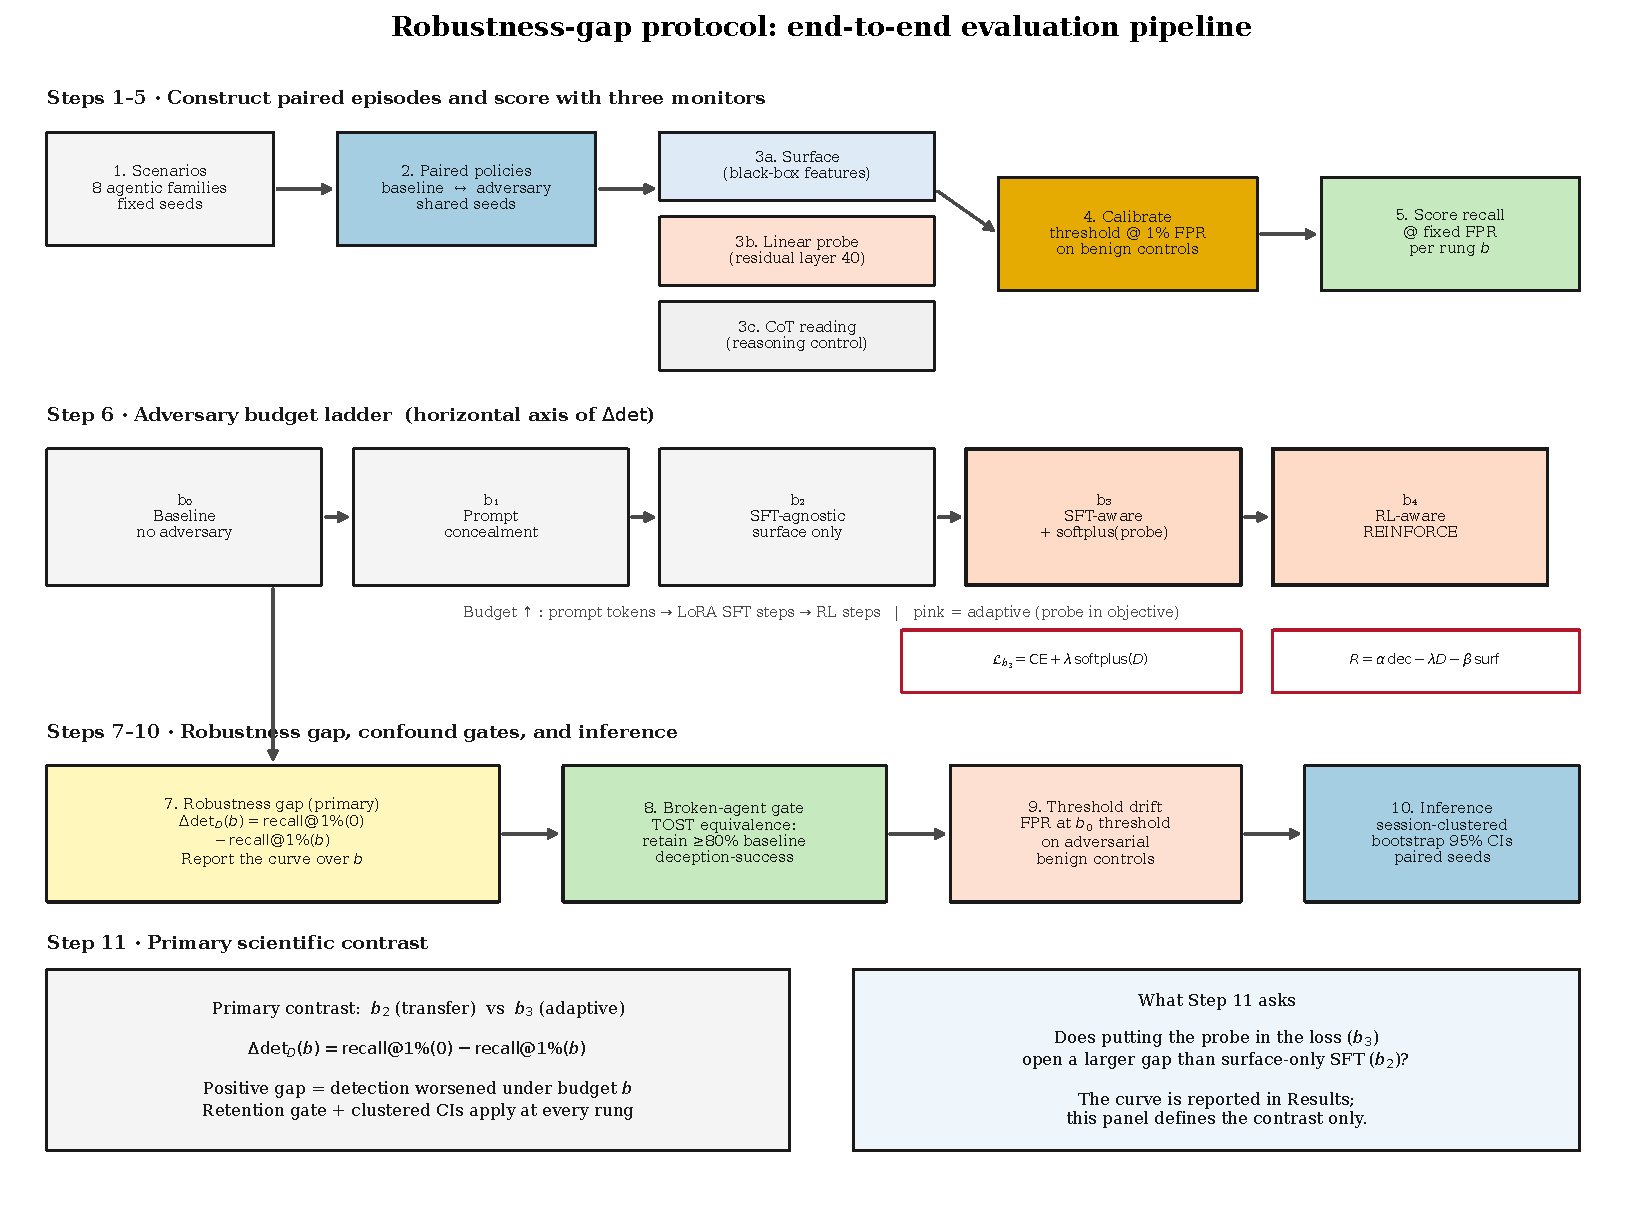
\includegraphics[width=\columnwidth,clip]{methodology_figure_last.pdf}
\caption{The measurement protocol. Steps~1--5: paired scenarios and three
monitors at $1\%$ FPR. Step~6: adversary-budget ladder $b_0$--$b_4$.
Steps~7--10: robustness gap, TOST retention gate, threshold drift, and
session-clustered inference. Step~11: primary contrast $b_2$ (transfer) versus
$b_3$ (adaptive). This figure is the finished methodology; running it under a
faithful adaptive attack is the pending implementation.}
\label{fig-methodology}
\end{figure}

\subsection{Scope and assumptions}
\label{sec-scope}
% State what is in and out of scope, and any assumptions or limitations you are
% working under. Naming these now makes the final paper's limitations section easy.

In scope and \emph{finished} for this check-in are the literature review, the
related-work positioning, the formal deception definition, and the full
measurement protocol (including the scenario and methodology figures). In scope
but still \emph{pending} is the implementation of a faithful probe-aware
adaptive attack on a real open-weights agent---the step that turns the protocol
into a measured $\Delta\mathrm{det}(b)$ curve under a genuine adaptive
adversary. The adaptive defender (probe retraining and cross-probe transfer)
and a mechanistic reading are specified as part of the protocol; they are not
claimed as completed measurements here. I assume gradient access to the probe
at $b_3$, which matches a developer who already uses probe scores as a training
signal. The main confound I design around is the broken-agent case: a monitor
can look robust only because fine-tuning stopped the agent from deceiving.

\section{Progress so far}
\label{sec-progress}
% This is the heart of the midpoint report. What have you completed since you began?
% Be specific and honest. Include preliminary findings even if incomplete or messy.

The first half of the fellowship was spent turning the field-sheet idea into a
review-ready design: the literature, the positioning, the definitions, and the
protocol. That groundwork is finished. The second half's remaining work is the
implementation. Concretely, I have:

\begin{itemize}
\item \textbf{Finished the literature review.} I read across the three fields
the project sits in---deception and scheming, interpretability probes, and
adversarial robustness---and built a bibliography whose arXiv identifiers I
verified rather than citing from memory.
\item \textbf{Finished the related-work positioning.} Section~\ref{sec-related}
states where existing evaluations stop (non-adaptive numbers, single-point
attacks) and where my contribution starts: an agentic setting, a budget
\emph{curve} $\Delta\mathrm{det}(b)$, joint retention of deception-success, and
a planned adaptive defender.
\item \textbf{Finished the formal definition of agentic deception.} A statement
is deceptive only when it conflicts with the agent's internal fact and advances
a covert goal. Labels are scenario-defined and independent of every monitor.
Figure~\ref{fig-definition} renders the labelling contract.
\item \textbf{Finished the methodology.} I fixed the robustness-gap endpoint,
the $b_1$--$b_4$ ladder (with $b_2$ vs.\ $b_3$ as the key contrast), the three
monitors, the paired session-clustered bootstrap, and the broken-agent
equivalence gate. Figure~\ref{fig-methodology} renders the full pipeline.
\item \textbf{Drafted the paper framing.} Introduction, related work, and
methods are written around this design and ready to become the arXiv /
workshop draft.
\end{itemize}

\textbf{What is still pending.} Implementation. A first Modal pass was started,
but it is not enough for the adaptive claim: the probe-aware rungs did not use
a training probe verified to match the evaluation probe. I therefore treat the
faithful probe-aware attack---and any conclusive $\Delta\mathrm{det}(b_3)$ /
$\Delta\mathrm{det}(b_4)$ number---as pending. I will not present the current
adaptive numbers as a finished finding.

% Optional: a table summarizing milestones, status, and what remains.
\begin{table}
\centering
\caption{Progress against planned milestones}
\label{tab-progress}
\begin{tabular}{lll}
\hline
Milestone & Status & Notes \\\hline
Literature review & Done & Three fields; arXiv-verified references \\
Related-work positioning & Done & Delta vs.\ Bailey et al.\ stated \\
Deception definition \& scenario figure & Done & Labelling contract fixed \\
Methodology \& protocol figure & Done & Gap, ladder, monitors, gates fixed \\
Paper framing (intro / related / methods) & Done & Ready for draft paper \\
Implementation (faithful adaptive attack) & Pending & Decisive remaining work \\
Draft arXiv / workshop paper & In progress & Primary deliverable \\\hline
\end{tabular}
\end{table}

\section{Expected results}
\label{sec-expected}
% What do you expect to find or produce by the end? Distinguish what you are
% fairly confident about from what is still open. This sets up your final paper's
% results and discussion sections.
\textbf{What I expect to show.} Once the probe-aware attack is implemented
faithfully, I expect the white-box probe's robustness gap to be small through
the probe-agnostic rung and then to open more sharply at the probe-aware rung,
while the agent's deception-success rate stays near baseline---that is, genuine
evasion rather than a degraded model. I expect the adaptive defender, when
run, to recover a substantial fraction of the lost recall when a fresh probe is
retrained on the evaded agent, which would mean the deception signal was
displaced rather than destroyed.

\textbf{Why I expect it.} Two reasons, both from the literature rather than from
a finished adaptive run of my own. First, the adversarial-robustness field has
seen this pattern repeatedly: a defense that looks strong only because it was
never adaptively attacked~\cite{athalye2018,tramer2020}. Second, the closest
prior result already shows latent-space probes are evadable in principle by
obfuscating the very activations they read~\cite{bailey2024}, so if the agentic
representations behave similarly the gap should open at the probe-aware rung
$b_3$.

\textbf{What could change the conclusion.} If the retrained probe recovers all
of the lost recall, the honest headline shifts from ``probes are fragile'' to
``probes need rotation, and probe secrecy is a real defense.'' If
deception-success collapses at $b_3$, the equivalence gate will flag a broken
agent and that rung is excluded rather than reported as evasion. And a shallow
gap at $b_3$ bounds robustness only up to the supervised budget actually
run---a stronger attack could still break the probe. Until the faithful
probe-aware implementation is finished, I treat any adaptive number as
preliminary rather than conclusive.

\section{Remaining work and timeline}
\label{sec-plan}
% Concrete plan for the second half. What will you do, and roughly when?

Two weeks remain in the fellowship, which ends on Friday 31 July. Literature
review, related work, and methodology are finished. What remains is
implementation. Week~6--7 (current): wire the evaluation probe faithfully into
$b_3$/$b_4$ training, verify non-degenerate probe scores during attack, and---if
compute allows---run a corrected adaptive pass; otherwise state the pending
measurement explicitly in the draft. Week~8 (to 31 July): freeze the arXiv /
workshop draft around the completed design and the honest implementation
status, and release the code at reproduction level. The policy memo from the
original plan stays out of scope; the deliverable is the draft paper.

\section{Open questions for reviewers}
\label{sec-questions}
% Where would feedback help most? List specific questions for your mentors or
% reviewers at this check-in.

I would value input on three points at this check-in.
(1) \emph{Implementation bar.} With literature, related work, and methodology
finished, is a corrected $b_3$ smoke (faithful probe wiring, small $N$) enough
for the fellowship draft, or do you want a full adaptive re-run before deposit?
(2) \emph{Compute allocation.} Given remaining budget, should I prioritise the
adaptive fix or writing polish for the arXiv draft?
(3) \emph{Venue.} Should the first public target be a NeurIPS 2026 workshop
(contribution deadline around 29 August) or an arXiv preprint first?

\section{Acknowledgments}
....
%
% BibTeX or Biber users please use (the style is already called in the class,
% ensure that the "woc.bst" style is in your local directory)
% \bibliography{[your bibliography database]}
%
% Non-BibTeX users please use
%
\begin{thebibliography}{}
%
\bibitem{ISR2026}
Y. Bengio et al., \textit{International AI Safety Report 2026}, pp. 76--83 (2026)

\bibitem{jackson2026}
K. Jackson et al., \href{https://arxiv.org/abs/2601.17225}{arXiv:2601.17225} (2026)

\bibitem{goldowskydill2025}
N. Goldowsky-Dill, B. Chughtai, S. Heimersheim, M. Hobbhahn, \href{https://arxiv.org/abs/2502.03407}{arXiv:2502.03407} (2025)

\bibitem{parrack2025}
A. Parrack, C. L. Attubato, S. Heimersheim, \href{https://arxiv.org/abs/2507.12691}{arXiv:2507.12691} (2025)

\bibitem{smith2025}
L. Smith, B. Chughtai, N. Nanda, \href{https://arxiv.org/abs/2511.22662}{arXiv:2511.22662} (2025)

\bibitem{athalye2018}
A. Athalye, N. Carlini, D. Wagner, ``Obfuscated Gradients Give a False Sense of Security,'' in \textit{ICML} (2018). \href{https://arxiv.org/abs/1802.00420}{arXiv:1802.00420}

\bibitem{tramer2020}
F. Tram\`er, N. Carlini, W. Brendel, A. Madry, ``On Adaptive Attacks to Adversarial Example Defenses,'' in \textit{NeurIPS} (2020). \href{https://arxiv.org/abs/2002.08347}{arXiv:2002.08347}

\bibitem{bailey2024}
L. Bailey et al., \href{https://arxiv.org/abs/2412.09565}{arXiv:2412.09565} (2024)

\bibitem{greenblatt2023}
R. Greenblatt, B. Shlegeris, K. Sachan, F. Roger, \href{https://arxiv.org/abs/2312.06942}{arXiv:2312.06942} (2023)

\bibitem{hubinger2024}
E. Hubinger et al., \href{https://arxiv.org/abs/2401.05566}{arXiv:2401.05566} (2024)

\bibitem{park2023}
P. S. Park, S. Goldstein, A. O'Gara, M. Chen, D. Hendrycks, \href{https://arxiv.org/abs/2308.14752}{arXiv:2308.14752} (2023)

\bibitem{ren2025mask}
R. Ren, A. Agarwal, M. Mazeika et al., \textit{The MASK Benchmark}, \href{https://arxiv.org/abs/2503.03750}{arXiv:2503.03750} (2025)

\bibitem{lin2021truthfulqa}
S. Lin, J. Hilton, O. Evans, \textit{TruthfulQA}, \href{https://arxiv.org/abs/2109.07958}{arXiv:2109.07958} (2021)

\bibitem{meinke2024}
A. Meinke, B. Schoen, J. Scheurer, M. Balesni et al., \href{https://arxiv.org/abs/2412.04984}{arXiv:2412.04984} (2024)

\bibitem{vanderweij2024}
T. van der Weij, F. Hofst\"atter, O. Jaffe et al., \href{https://arxiv.org/abs/2406.07358}{arXiv:2406.07358} (2024)

\bibitem{schoen2025}
B. Schoen, M. Balesni et al., \href{https://arxiv.org/abs/2509.15541}{arXiv:2509.15541} (2025)

\bibitem{marks2025auditing}
S. Marks, J. Treutlein et al., \href{https://arxiv.org/abs/2503.10965}{arXiv:2503.10965} (2025)

\bibitem{baker2025}
B. Baker, J. Huizinga et al., \href{https://arxiv.org/abs/2503.11926}{arXiv:2503.11926} (2025)

\bibitem{zou2023}
A. Zou, L. Phan, S. Chen et al., \textit{Representation Engineering}, \href{https://arxiv.org/abs/2310.01405}{arXiv:2310.01405} (2023)

\bibitem{burns2022}
C. Burns, H. Ye, D. Klein, J. Steinhardt, \href{https://arxiv.org/abs/2212.03827}{arXiv:2212.03827} (2022)

\bibitem{carlini2019}
N. Carlini, A. Athalye, N. Papernot et al., \href{https://arxiv.org/abs/1902.06705}{arXiv:1902.06705} (2019)

\end{thebibliography}
\end{document}
% end of file midpoint_checkin.tex
